\documentclass[mathserif, aspectratio=169]{beamer}
\usetheme{odenpecos}
\setbeamertemplate{itemize/enumerate body begin}{\fontsize{8.8}{9}\selectfont}
\setbeamertemplate{itemize/enumerate subbody begin}{\fontsize{7.5}{8}\selectfont}
\setbeamertemplate{itemize/enumerate subsubbody begin}{\fontsize{7.5}{8}\selectfont}

% default search path for figures
\graphicspath{{./shared_figures/}{./figures/}}

\newcommand{\zapspace}{\topsep=0pt\partopsep=0pt\itemsep=0pt\parskip=0pt}

\usepackage{multicol}
\usepackage{pict2e}
\usepackage{esdiff}
\usepackage{multimedia}
\usepackage{verbatim}
\usepackage{mhchem}

\usepackage[percent]{overpic}
\usepackage[absolute,overlay]{textpos}

\newcommand{\overbar}[1]{\mkern 1.5mu\overline{\mkern-1.5mu#1\mkern-1.5mu}\mkern 1.5mu}
\newcommand{\pp}[2]{\frac{\partial #1}{\partial #2}}
\newcommand{\dd}[2]{\frac{d #1}{d #2}}
\newcommand{\DD}[2]{\frac{D #1}{D #2}}
\newcommand{\mm}{\mathbf{minmod}}
\def\etal{{\it et al~}}
\newcommand{\be}{\begin{eqnarray}}
\newcommand{\ee}{\end{eqnarray}}
\newcommand{\mbb}[1]{\mathbb{#1}} % math blackboard bold
\newcommand{\mcal}[1]{\mathcal{#1}} % math blackboard bold
\newcommand{\mbf}[1]{\mathbf{#1}} % math bold face (for vectors)
\newcommand{\sbf}[1]{\boldsymbol{#1}} % bold face for symbols
\newcommand{\jump}[1]{\llbracket #1 \rrbracket} % jump operator
\newcommand{\avg}[1]{\langle #1 \rangle} % average operator
\newcommand{\rarrow}{\rightarrow}
\newcommand{\Rarrow}{\Rightarrow}
\newcommand{\LRarrow}{\Leftrightarrow}
\newcommand{\vvvert}{|\kern-1pt|\kern-1pt|}
\newcommand{\enorm}[1]{\vvvert #1 \vvvert}
\newcommand{\nutil}{\tilde{\nu}}
\newcommand{\Var}{\mathrm{Var}}
\newcommand{\Cov}{\mathrm{Cov}}


\definecolor{MyDarkGreen}{rgb}{0,0.45,0.08}
\newcommand{\myred}[1]{{\color{red} #1}}
\newcommand{\myblue}[1]{{\color{blue} #1}}
\newcommand{\mygreen}[1]{{\color{MyDarkGreen} #1}}

\newcommand{\sa}{\nu_{\mathrm{sa}}}
\newcommand{\tep}{\tilde{\epsilon}}
\newcommand{\Ssd}{\mathcal{S}} % source term due to slow derivative
\newcommand{\ud}{\,\mathrm{d}}

\newcommand{\Mach}[1]{\ensuremath{\mbox{Ma}_{#1}}}
\newcommand{\Reynolds}{\ensuremath{\mathit{Re}}}
\newcommand{\DensityRat}{\ensuremath{\mathit{DR}}}
\newcommand{\BlowRat}{\ensuremath{\mbox{BR}}}
\newcommand{\VelRat}{\ensuremath{\mathit{VR}}}
\newcommand{\Tau}{\ensuremath{\mathrm{T}}}

\newcommand{\wall}     {\ensuremath{\mathrm{w}}}   % wall subindex
\newcommand{\awall}    {\ensuremath{\mathrm{aw}}}  % adiabatic wall subindex

\newcommand{\commentout}[1]{}

\newcommand{\vect}[1]{\boldsymbol{#1}}
\usepackage{mleftright}
\newcommand{\of}[1]{\mleft( #1 \mright)}
\newcommand{\vth}{v_{\textrm{th}}}
\newcommand{\reals}{\mathbb{R}}
\newcommand{\myint}{\int\limits}
\newcommand{\ddt}[1]{\partial_t #1}
\newcommand{\RR}{\mathbb{R}}
\newcommand{\vr}{v}
%\newcommand{\vtheta}{\theta_{\vect{v}}}
%\newcommand{\vphi}{\varphi_{\vect{v}}}
%\newcommand{\vr}{v_{r}}
\newcommand{\vtheta}{v_{\theta}}
\newcommand{\vphi}{v_{\varphi}}
\newcommand{\vomega}{v_{\omega}}
\newcommand{\vrunit}{\hat{\vect{v}}_{r}}
\newcommand{\vthetaunit}{\hat{\vect{v}}_{\theta}}
\newcommand{\vphiunit}{\hat{\vect{v}}_{\varphi}}
\DeclareMathOperator{\variance}{Var}

\begin{document}
% disable nav
\setbeamertemplate{navigation symbols}{}

% ---------------------------------------------------------------
% Oden/Pecos title page

%\hoffset=.16in
%
%\begin{frame}[plain,t]{}
%\makeatletter
%%\vspace*{0.85cm}
%%\vspace*{0.65cm}
%\includegraphics[height=0.9in,trim=50 40 40 0, clip]{PMSc_159_university_formal_horizontal.pdf} \newline
%%\vspace*{0.3cm}
%\begin{columns}[T,onlytextwidth]
%\column{.8\textwidth}
%{\bf \color{burntorange} \fontfamily{bch}\selectfont 
%% -- Set talk title here
%Solving the Boltzmann equation for electron kinetics using Petrov-Galerkin approach
%% --
%}
%\end{columns}
%\vspace*{.15cm}
%\rule{.8\textwidth}{0.6pt} \newline
%
%\vspace*{0.05cm}
%\setstretch{0.65}
%{\fontfamily{phv}\selectfont
%  { \scriptsize
%    % -- define presenter, authors here
%    Milinda Fernando, Daniil Bochkov, Todd Oliver, George Biros\newline
%    % --
%  }
%  {\color{burntorange} \tiny
%    % -- define role, meeting event, location, etc
%    Year-1 Review $\cdot$ August, 2021 $\cdot$ Austin, TX
%    % --
%  }
%}
%
%\vspace*{1cm}
%%\includegraphics[height=0.3in]{figures/pecos_orange1.png}
%\begin{columns}
%\begin{column}{0.8\linewidth}
%\includegraphics[height=0.5in]{oden_pecos_2020_wordmark.png}\\
%{\scriptsize \url{https://pecos.oden.utexas.edu}}
%\end{column}
%
%\begin{column}{0.2\linewidth}
%\includegraphics[height=0.6in]{psaap3-logo.png}
%\end{column}
%\end{columns}
%
%\end{frame}
%\hoffset=0in
% -- end title slide ---------------------------------------------


\begin{frame}
\begin{itemize}
\item Advection equation
\begin{align*}
\partial_t f - \vect{E} \cdot \nabla_{\vect{v }}f = 0
\end{align*}
\item In spherical coordinates
\begin{align*}
\nabla_{\vect{v}} 
= \vrunit \frac{\partial}{\partial \vr}
+ \vthetaunit \frac{1}{\vr} \frac{\partial}{\partial \vtheta}
+ \vphiunit \frac{1}{\vr \sin\of{\vtheta}} \frac{\partial}{\partial \vphi}
\end{align*}
\begin{align*}
\vect{E} 
= E \hat{\vect{z}} 
= E \left( \cos\of{\vtheta} \vrunit - \sin\of{\vtheta} \vthetaunit \right)
\end{align*}
\begin{align*}
\vect{E}\cdot \nabla_{\vect{v}} f
= E 
\left( \cos\of{\vtheta} \frac{\partial f}{\partial \vr} 
- \sin\of{\vtheta} \frac{1}{\vr} \frac{\partial f}{\partial \vtheta} \right)
\end{align*}

\end{itemize}
%
\end{frame}

\begin{frame}

\begin{itemize}

\item Expansion in terms of B-splines and spherical harmonics
\begin{align*}
f = \sum_{klm} h_{klm} P_kl\of{\textstyle\frac{v}{\vth}} Y_{lm}\of{\vtheta,\vphi} \\
\end{align*}
To minimize the ill-conditioning  of the mass matrix, we write, 
\begin{align}
P_{kl}\of{\textstyle\frac{v}{\vth}} = \left(\textstyle\frac{v}{\vth}\right)^{max(l-k,0)} B_k\of{\textstyle\frac{v}{\vth}}
\end{align}


\item  Projection:
\begin{align*}
\myint_{\reals^3} \Bigg( \partial_t f - \vect{E} \cdot \nabla_{\vect{v }}f = 0 \Bigg) P_{pq}\of{\textstyle\frac{v}{\vth}} Y_{qs}\of{\vtheta,\vphi} \ud\vect{v} \ud\vomega
\end{align*}

\item Resulting system of ODEs:
\begin{align*}
\partial_t h_{pqs}\of{t} = \sum_{k,l,m}  \epsilon_{pqsklm} h_{klm}\of{t}
\end{align*}
\end{itemize}
%
\end{frame}

\begin{frame}
\frametitle{\small Convergence test ($N_r = 32$ is fixed, $l_{\max}$ is increasing)}
\begin{figure}
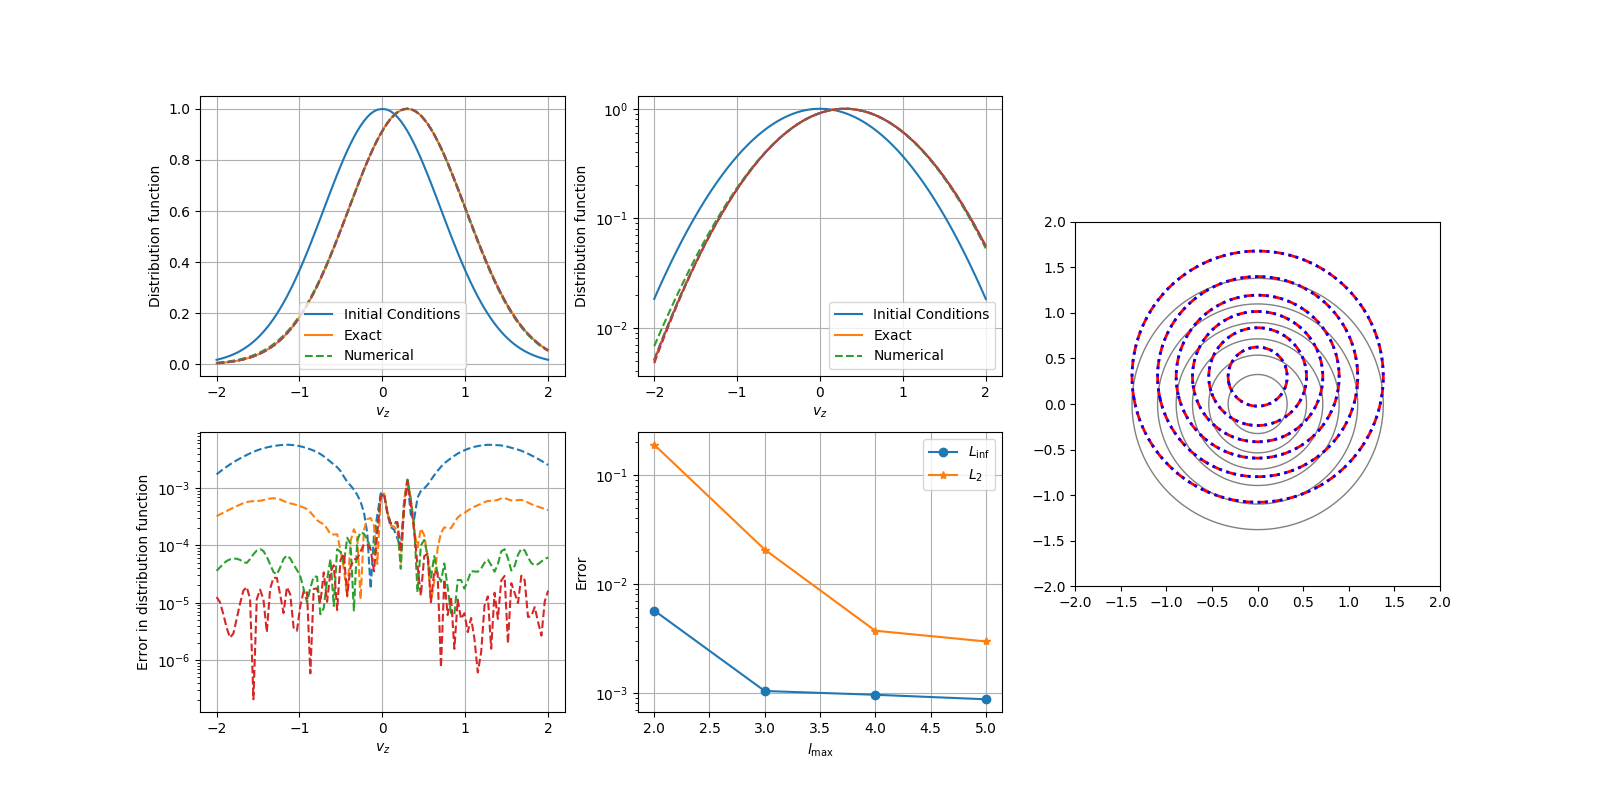
\includegraphics[width=0.9\textwidth]{figures/splines/nr_32_to_32_lmax_2_to_5.png}
\end{figure}
\end{frame}

\begin{frame}
\frametitle{\small Convergence test ($N_r$ is increasing, $l_{\max} = 5$ is fixed)}
\begin{center}
%\begin{itemize}
%\item 
%$\vect{E} = \text{const} \rightarrow f\of{t,\vect{v}} = f\of{0, \vect{v} + \vect{E}t}$
%\item $N_r = 32$ is fixed, $l_{\max}$ is increasing
%\end{itemize}
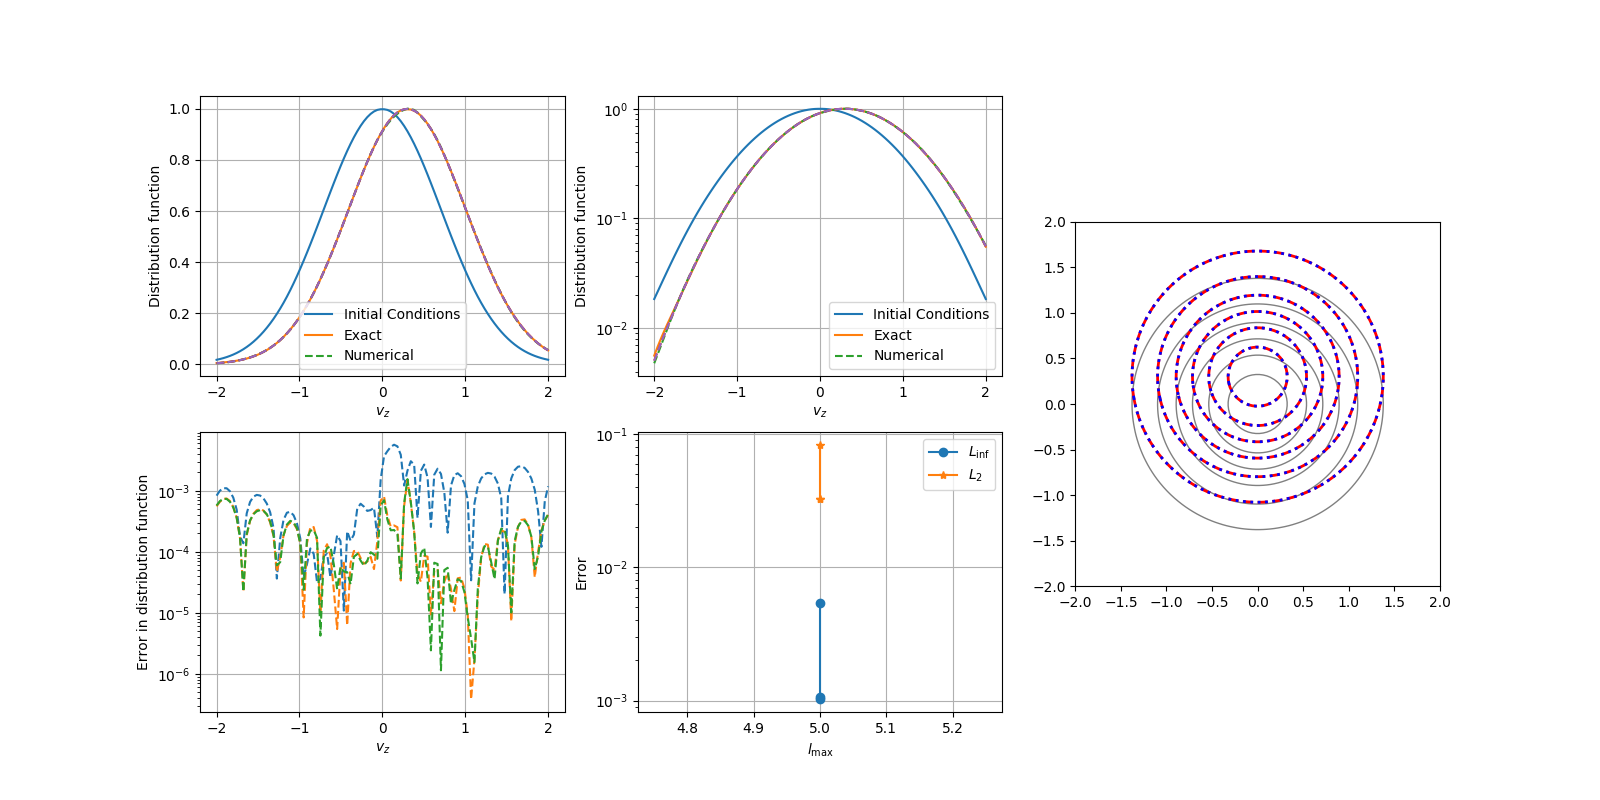
\includegraphics[width=0.9\textwidth]{figures/splines/nr_16_to_64_lmax_5_to_5.png}
\end{center}
\end{frame}

\begin{frame}
\frametitle{\small Convergence test ($N_r$ is increasing, $l_{\max}$ is increasing)}
\begin{center}
%\begin{itemize}
%\item 
%$\vect{E} = \text{const} \rightarrow f\of{t,\vect{v}} = f\of{0, \vect{v} + \vect{E}t}$
%\item $N_r = 32$ is fixed, $l_{\max}$ is increasing
%\end{itemize}
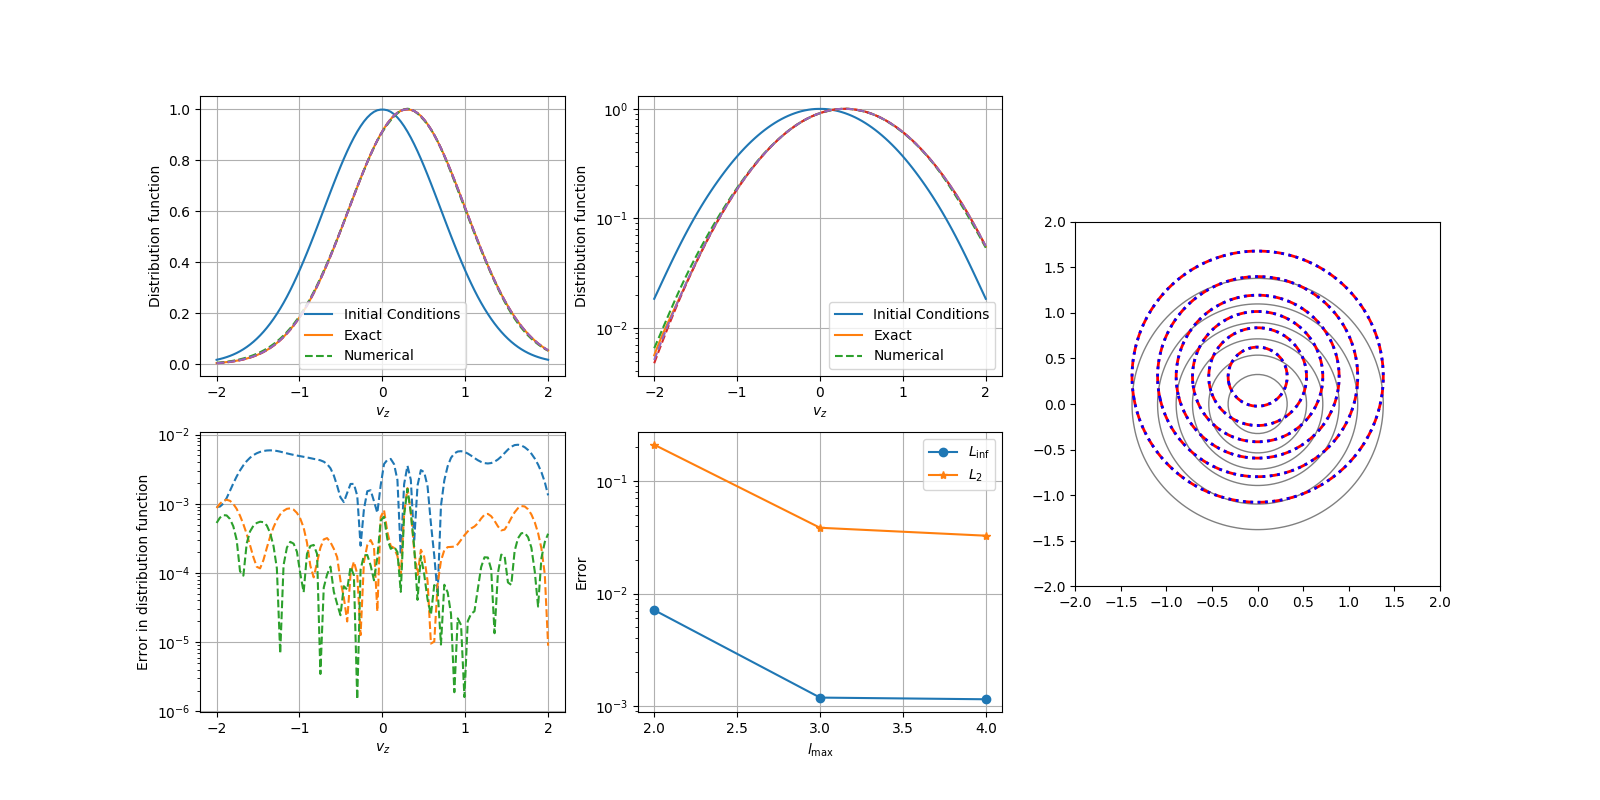
\includegraphics[width=0.9\textwidth]{figures/splines/nr_16_to_64_lmax_2_to_4.png}
\end{center}
\end{frame}

\begin{frame}{Mass matrix: conditioning issue}
	\begin{itemize}
		\item B-splines are placed, $[0,0,\cdots, t_0, t_1, \cdots, t_n]$
		\item To capture the peak well we need more knots close to $v=0$. 
		\item When $t_0 \rightarrow 0$, $M_{0j} \rightarrow [0,\cdots,0]$.
		\item Also conditioning issues with the $x^l$ factor for $P_{kl}$
	\end{itemize}
	
\end{frame}



%\begin{frame}
%\frametitle{\small Convergence test ($N_r = 16$ is fixed, $l_{\max}$ is increasing)}
%\begin{center}
%%\begin{itemize}
%%\item 
%%$\vect{E} = \text{const} \rightarrow f\of{t,\vect{v}} = f\of{0, \vect{v} + \vect{E}t}$
%%\item $N_r = 32$ is fixed, $l_{\max}$ is increasing
%%\end{itemize}
%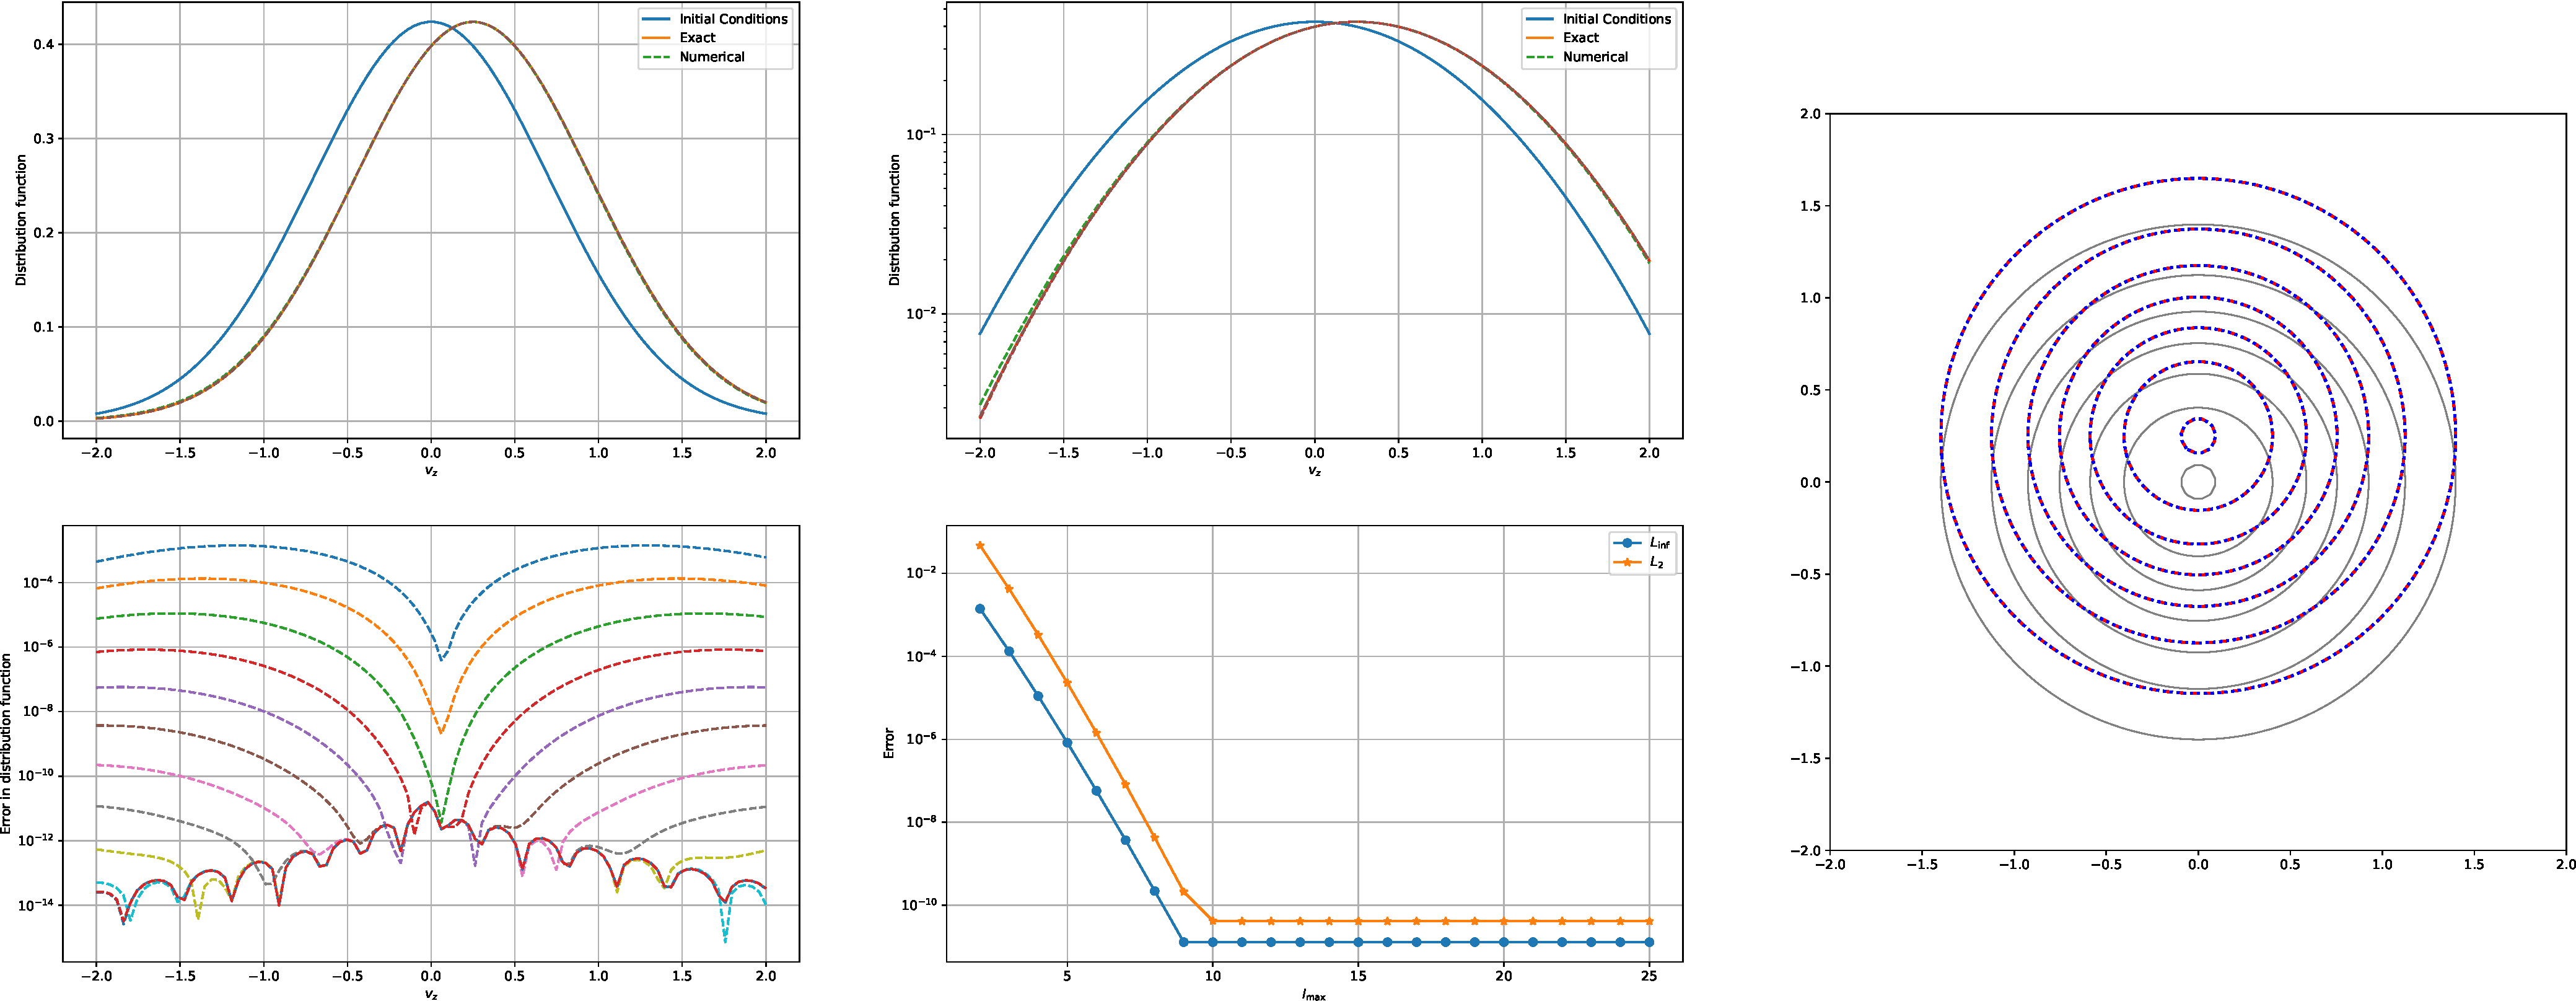
\includegraphics[width=0.99\textwidth]{figures/advection_operator_changing_lmax_0_25}
%\end{center}
%\end{frame}
%
%\begin{frame}
%\frametitle{\small Convergence test ($N_r = 16$ is fixed, $l_{\max}$ is increasing)}
%\begin{center}
%%\begin{itemize}
%%\item 
%%$\vect{E} = \text{const} \rightarrow f\of{t,\vect{v}} = f\of{0, \vect{v} + \vect{E}t}$
%%\item $N_r = 32$ is fixed, $l_{\max}$ is increasing
%%\end{itemize}
%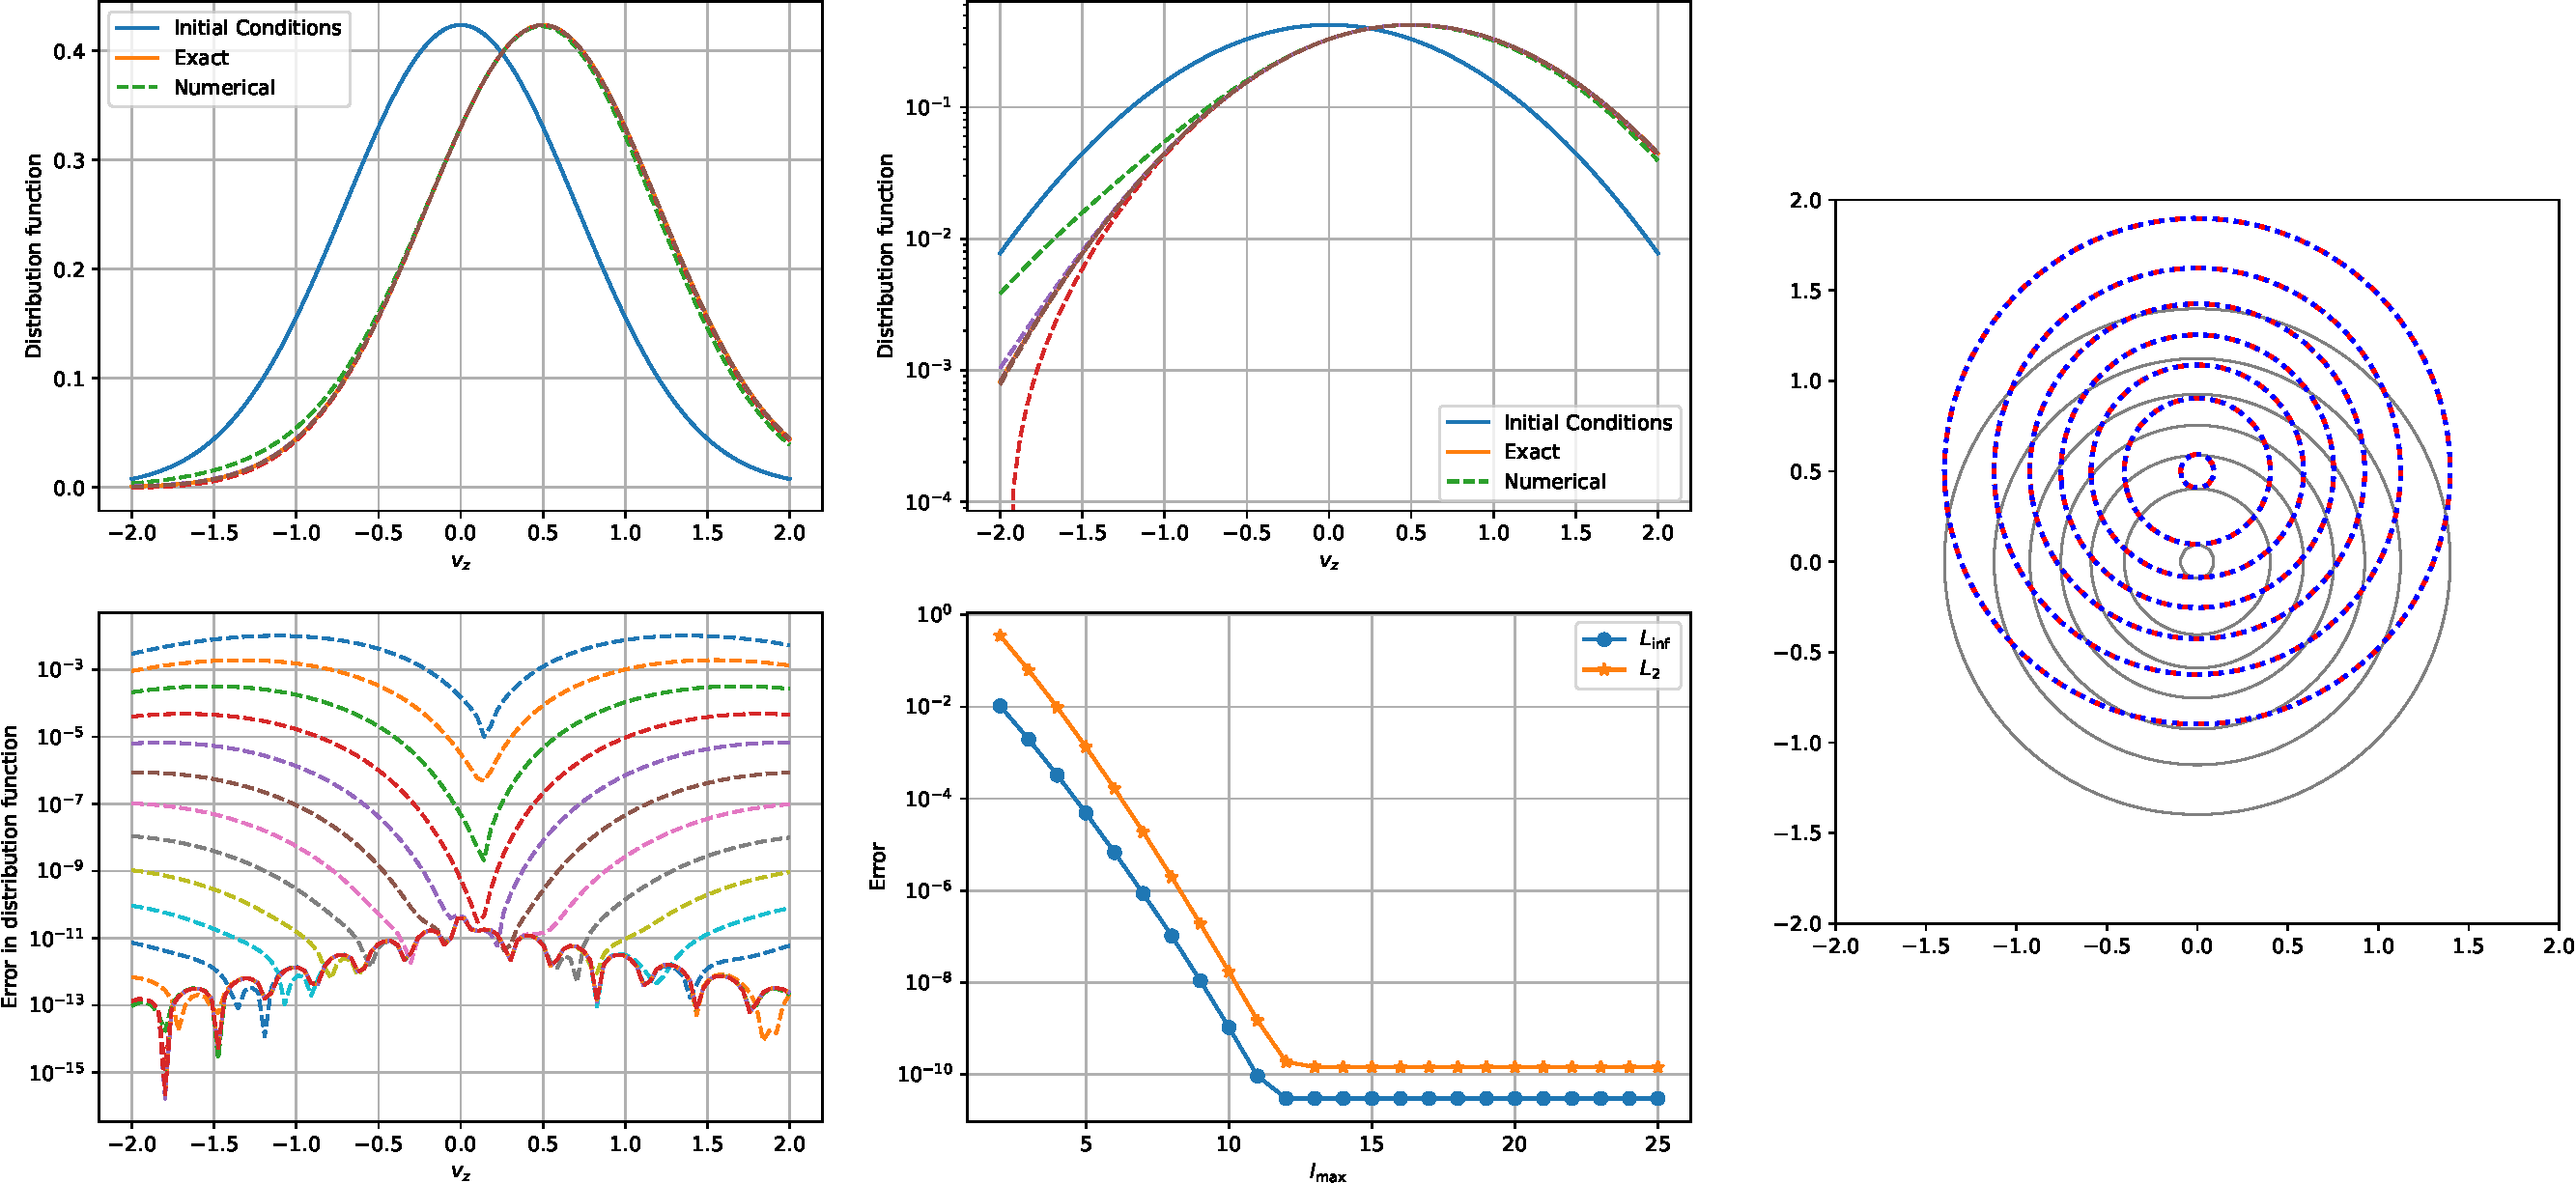
\includegraphics[width=0.99\textwidth]{figures/advection_operator_changing_lmax}
%\end{center}
%\end{frame}

%===============================================================================
\end{document}

